\chapter{Experimental setup}
\label{chap:detector}
%20-25 pages.
This chapter provides a description of the various components of the Large 
Hadron Collider and the CMS detector. The techniques employed to reconstruct 
the particles that are produced in the proton collisions are discussed, as well 
as the event simulation method.

\section{The Large Hadron Collider}
%CERN and LHC. Franco-Swiss border. 26 km. 100m underground. 
%Largest and most powerful.
The LHC at CERN is a circular accelerator and collider of protons (and lead 
ions). It is 27~kilometres in circumference, and is situated on the border 
between France and Switzerland near Geneva, approximately 100~metres 
underground. It was designed to investigate the standard model and search for 
new physics. %The Higgs boson was successfully discovered at the LHC in 
%2012~\cite{higgs-cms,higgs-atlas}.

\begin{figure}
\centering
% trim={left bottom right top}
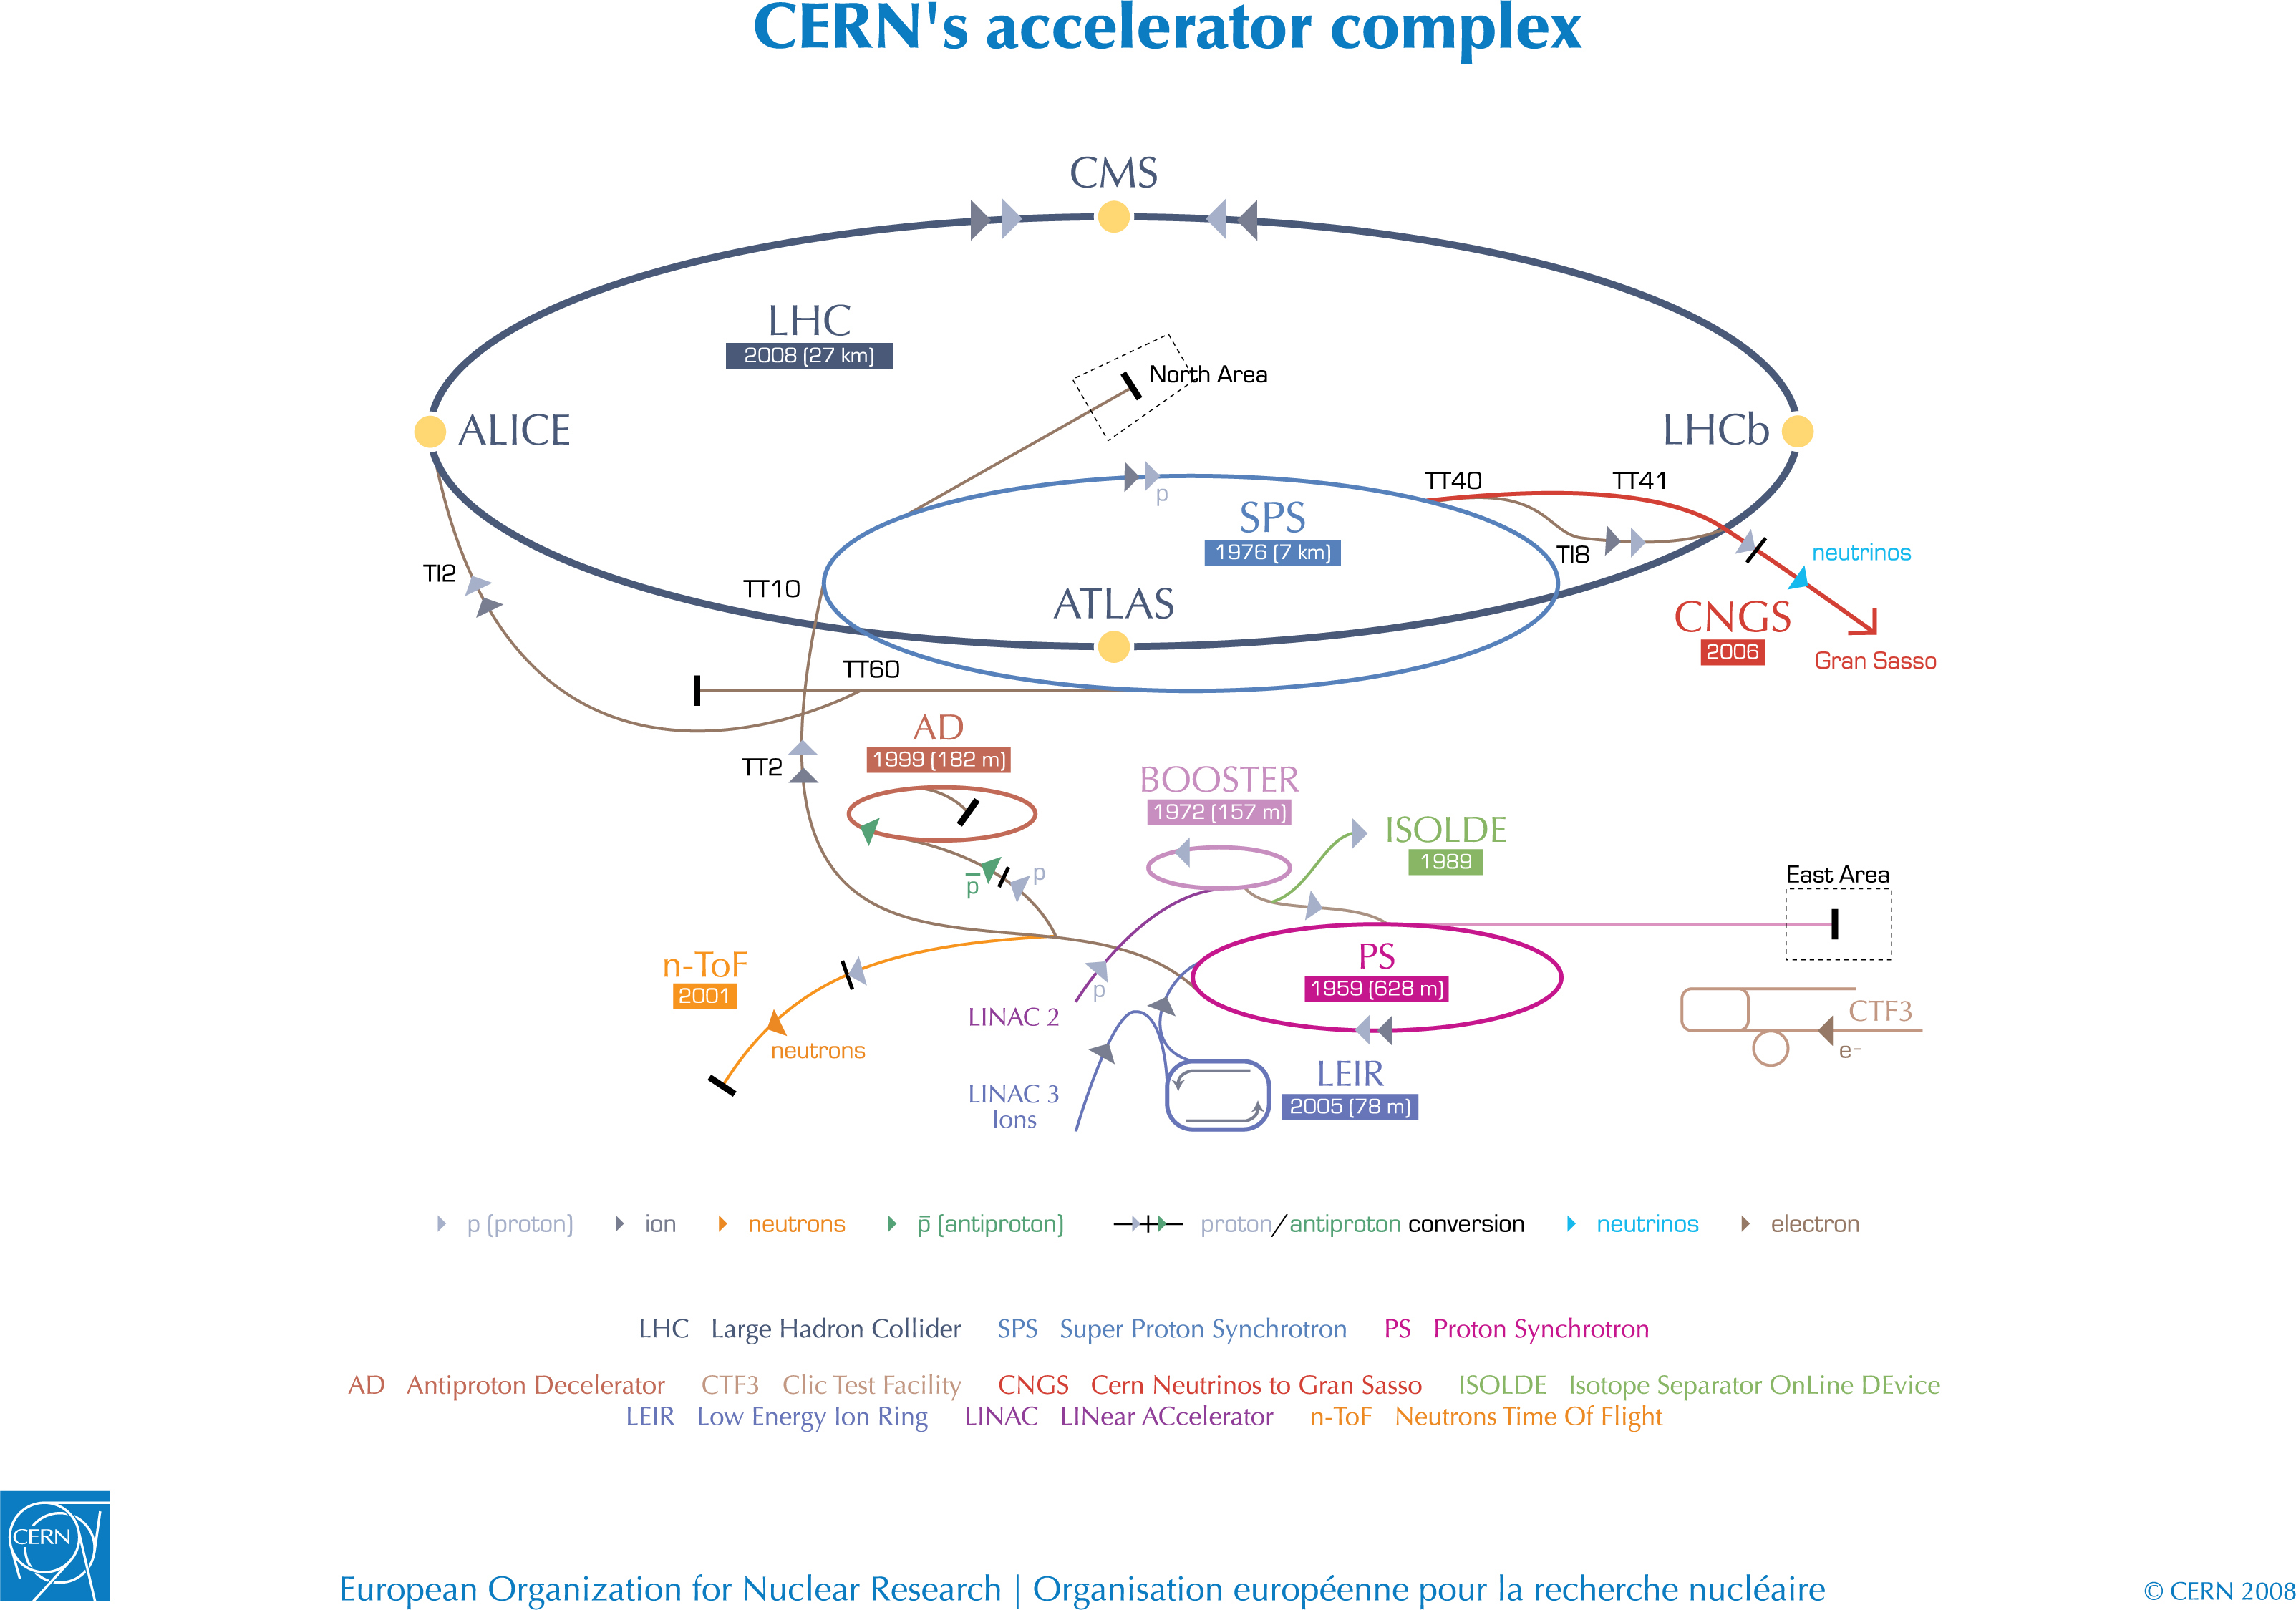
\includegraphics[width=1\textwidth, trim={2cm 5cm 2cm 1.5cm}, 
clip]{figs/detector/lhc-complex}
\caption{The accelerator complex at CERN leading to the LHC~\cite{lhc-complex}. 
The various accelerators (LINAC 2, PSB, PS, SPS, LHC) and detectors (CMS, 
ATLAS, LHCb, ALICE) are described in the text.}
\label{fig:lhc-complex}
\end{figure}

%Accelerator complex: hydrogen, LINAC, PS, SPS, etc (show diagram).
%4 detectors/collision points.
The accelerator complex at CERN is illustrated in Fig.~\ref{fig:lhc-complex}. 
The particle acceleration occurs in various stages. First, hydrogen atoms from 
a gas bottle are stripped of their electrons and the resulting protons are 
accelerated to 50~MeV in the Linear Accelerator 2 (LINAC 2). These protons are 
then injected into the Proton Synchrotron Booster (PSB) to increase their 
energy to 1.4~GeV. This is followed by the Proton Synchrotron (PS), where the 
protons reach 25~GeV, and the Super Proton Synchrotron (SPS), which further 
accelerates them to 450~GeV. The protons then finally arrive at the LHC, where 
they are accelerated by radio frequency cavities up to an energy of 6.5~TeV, 
and are steered and focussed by superconducting magnets.
% dipole to steer, quadrupole to focus
% 1200 dipole magnets, 8 Tesla
% https://home.cern/about/engineering/radiofrequency-cavities
During this process, the protons are also collected into bunches of 
approximately 115~billion protons each that are 25~ns apart. The total number 
of proton bunches circulating within a given fill of the LHC is 2808.
% bunches are 30 cm long
% spatial separation is 7.5 m 

The LHC consists of two beam pipes in which the protons are circulated in 
opposite directions. The protons are made to collide at a centre of mass energy 
of 13~TeV at four points on the ring, where the CMS~\cite{cms}, 
ATLAS~\cite{atlas}, LHCb~\cite{lhcb} and ALICE~\cite{alice} detectors are 
situated. CMS and ATLAS are both general purpose detectors, while LHCb and 
ALICE are focussed on b-physics and heavy ion physics, respectively.
% CP violation via the decays of b hadrons

For a process with a production cross section $\sigma$, the expected number of 
events per unit time is related to the instantaneous luminosity $L$ by the 
relation:
\begin{equation}
\frac{\mathrm d N}{\mathrm d t} = \sigma L \, .
\end{equation}
The instantaneous luminosity is proportional to the number of proton bunches, 
the number of protons per bunch and the revolution frequency, and is inversely 
proportional to the transverse size of the beam~\cite{pdg12}. 
% transverse dimensions are 15 microns
For the 2016 running conditions, the average instantaneous luminosity of the 
LHC was approximately $10^{34}$~\lumiunits, which resulted in an average number 
of 
interactions per bunch crossing (referred to as pileup) of $\sim$20.
% plug in inelastic xs to get pileup events per ns, multiply by 25 (50) to get 
%pileup events per bunch crossing
The total expected number of events of a process in a certain time $T$ is given 
by:
\begin{equation}
N = \sigma \int_{0}^{T} L ~ \mathrm d t = \sigma L_\mathrm{int} \, ,
\end{equation}
where the integral of the instantaneous luminosity over this time is called the 
integrated luminosity $L_\mathrm{int}$, and is a measure of the amount of data 
collected.

%Luminosity (instantaneous/integrated) and cross section formulas 
%(Marco-Andrea/Pesaresi).
%Pileup 20 (formula/estimate using inelastic xs?). Minimum bias.
%Bunch spacing, number of bunches, number of protons per bunch (Marco-Andrea 
%table).
%History of Run1, shutdown, Run 2. Amount of data delivered.

\begin{comment}
Collider physics.
Used to search for new physics and discover Higgs boson.
Need very high energy to produce high mass particles and search for new physics 
(cf xs vs com).
(Compare to ep collider and fixed target).
Proton-proton (and ion) collisions.
Centre of mass energy. 
Describe run, fill, lumi section, instantaneous luminosity values.
\end{comment}

\section{The Compact Muon Solenoid}
%One of two multipurpose detectors. Used to search for new physics and discover 
%Higgs boson.
%Hermetic coverage (good for MET). 
%identify particles (electrons, photons, hadrons, muons) with high precision
% Give size and mass? MA: 22 meters long and about 15 meters in diameter, with 
%a weight of 12,500 metric tons [55]. Isn't it 14,000 tonnes? The complete 
%detector is 21 metres long, 15 metres wide and 15 metres high.
The CMS detector is one of the two general purpose detectors at the LHC along 
with ATLAS, and was designed with the main goal of searching for the Higgs 
boson as well as for new physics beyond the standard model. The detector is 
cylindrical 
and consists of several layers of subdetectors and a solenoid magnet that are 
used to track, identify and measure the energy of particles such as electrons, 
photons, muons and hadrons. 
It extends up to a pseudorapidity of $\etaabs \approx 5$, providing an almost 
complete coverage in solid angle. This is important when reconstructing the 
momentum of a weakly interacting particle via the `missing momentum' in an 
event.
The detector is approximately 22~m in length and 15~m in diameter, and weighs 
about 14,000 tonnes.
The layout of the CMS detector is shown in Fig.~\ref{fig:cms3d}, and a 
cross-sectional view is given in Fig.~\ref{fig:cms2d}, illustrating the various 
components of the detector, which will be described in this section.

\begin{figure}
\centering
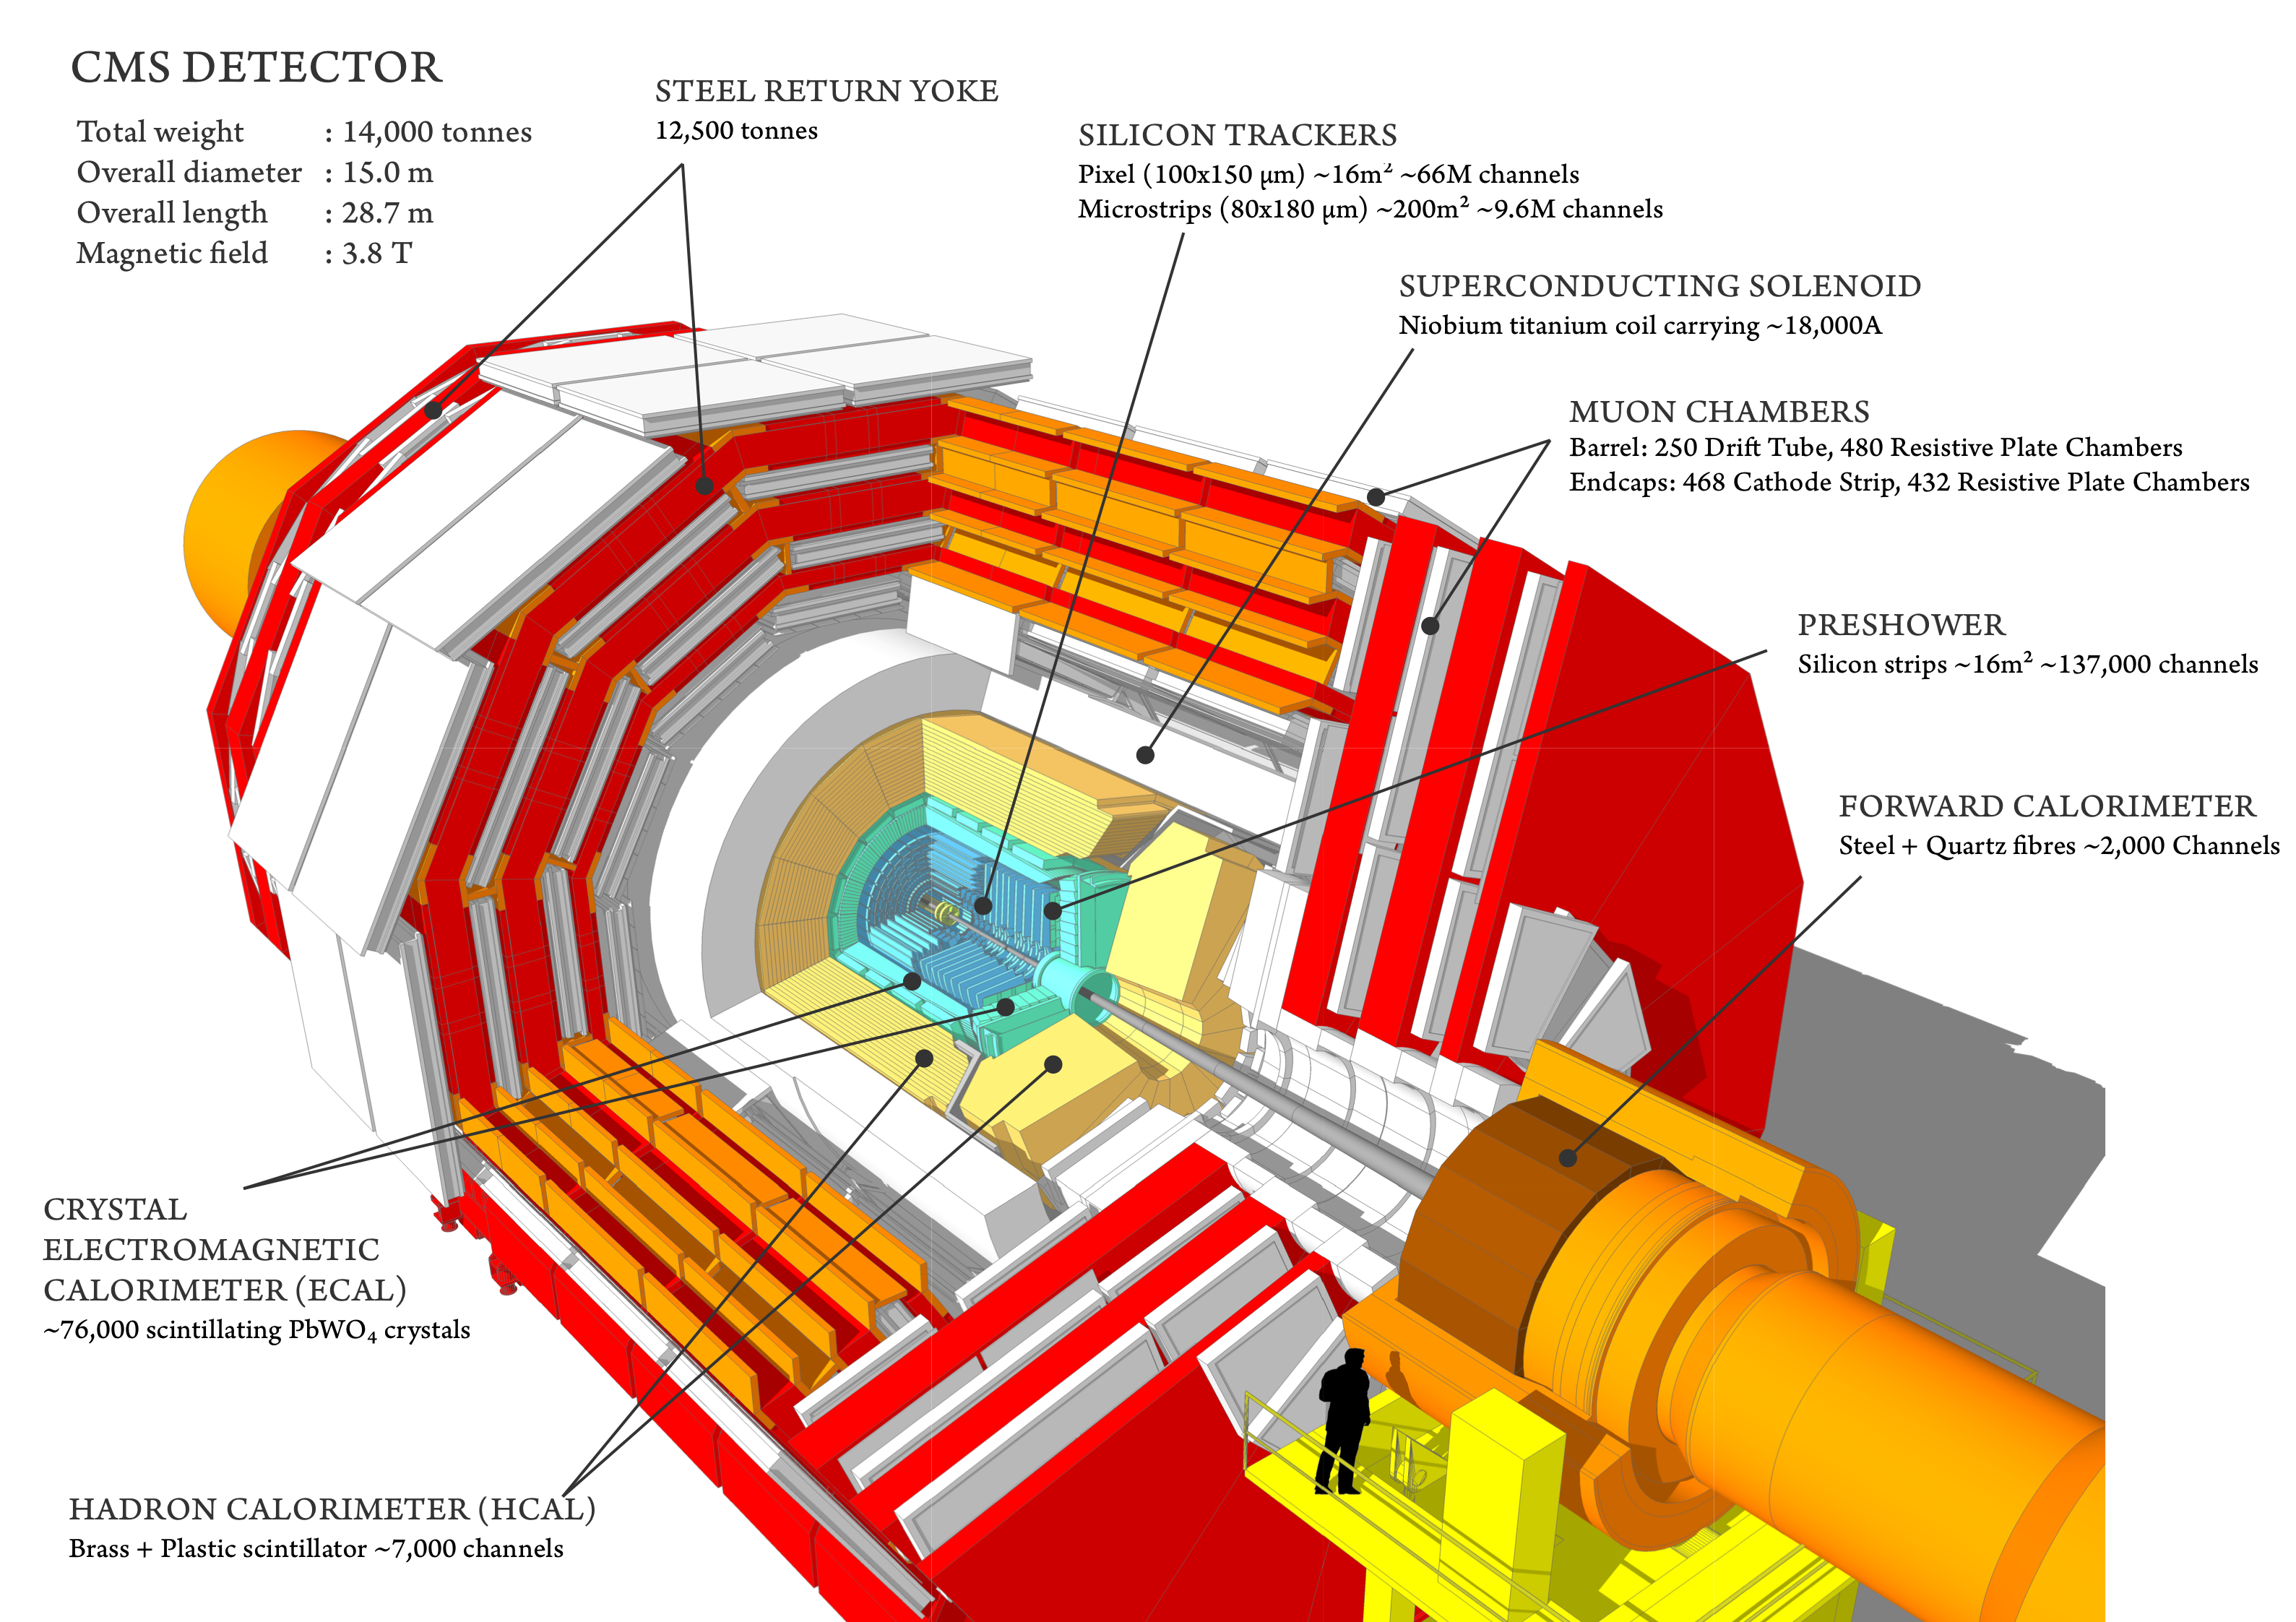
\includegraphics[width=1\textwidth]{figs/detector/cms3d}
\caption{Layout of the major components within the CMS detector. These are 
described in the text.}
\label{fig:cms3d}
\end{figure}
\begin{figure}
\centering
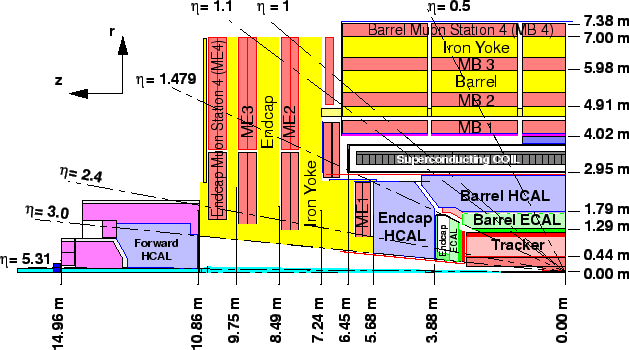
\includegraphics[width=0.8\textwidth]{figs/detector/cms2d.png}
\caption{One quarter cross-sectional view (in the $r$-$z$ plane) of the CMS 
detector, indicating lines of constant pseudorapidity and the dimensions of 
various components.}
\label{fig:cms2d}
\end{figure}

%Diagram.
%Overview of subdetectors. Magnet strength.
The tracker forms the first layer of the detector closest to the collision 
point. It is used to reconstruct the trajectories of charged particles within 
the magnetic field and measure their momenta. Following this is the 
electromagnetic calorimeter (ECAL), which is used to absorb and measure the 
energies of electrons and photons. The next layer is comprised of the hadronic 
calorimeter (HCAL), which detects the more penetrating hadrons. The 3.8~T 
superconducting solenoid surrounds the tracker and calorimeters. Muons are able 
to penetrate the magnet and calorimeters and are detected by the muon chambers, 
which are interspersed with the steel return yoke of the magnet in the 
outermost layer of the CMS enclosure.
%The data from all these subdetectors are read out by dedicated front end 
%electronics and passed through the CMS trigger system, which selects the most 
%promising data to be kept and stored for offline processing.
Finally, collision events of interest are read out by a trigger system.

%Coordinate system. Pseudorapidity. Cylindrical radius r.
% phi measured from x axis
A right-handed coordinate system is defined with the origin at the centre of 
the detector (which is approximately the interaction point). The $x$-axis lies 
horizontally towards the centre of the LHC ring, the 
$y$-axis points vertically upwards, and the $z$-axis points along the beam 
direction. An azimuthal angle $\phi$ is defined that lies in the transverse 
$x$-$y$ plane. The cylindrical radial coordinate is labelled $r$. A polar angle 
$\theta$ is measured from the $z$-axis and is related to 
pseudorapidity by $\eta = -\ln\left[\tan\left(\frac{\theta}{2}\right)\right]$.

\begin{comment}
The Compact Muon Solenoid (Fig. 1) is one of the two general purpose detectors,
along with ATLAS, at the LHC. It comprises a 13 m long, 4 T superconducting 
solenoid magnet within which lie a tracker, an electromagnetic calorimeter 
(ECAL) and a hadronic calorimeter (HCAL). Outside the magnet and within the 
return yoke lies the muon detection system.
The tracking system consists of an inner silicon pixel detector and an outer 
silicon microstrip tracker. The ECAL is constructed from crystals of lead 
tungstate and measures the energies of photons and electrons. The scintillation 
light produced by these particles as they pass through the crystals is detected 
by photodetectors. The HCAL consists of alternating brass absorbers and plastic 
scintillators. It surrounds the ECAL and detects the more penetrating hadrons. 
Muons are able to penetrate the magnet and calorimeters and are detected by 
chambers on the edge of the CMS enclosure. These consist of drift tubes and 
cathode strip chambers along with resistive plate chambers to provide a fast 
trigger response.
\end{comment}

%(maybe) Give extent (in radius) occupied by each subdetector as you go along.

\subsection{Tracker}
%How tracker works, ie electron-hole pairs (see Adam and MSci report).
%High radiation environment. Little material.
%Pixel tracker. (for vertices) r<20 cm
%Silicon strip tracker.
%TOB, TEC, etc. Their positions/extents.
%Momentum resolution, tracking efficiency, spatial resolution.
% follow MA and MSci report
The CMS tracker consists of a silicon pixel detector located closest to the 
interaction point ($r<20$~cm) and silicon strip detectors surrounding this. 
The more granular pixels are used to cope with the higher particle fluxes that 
are present near the interaction point, as well as to provide a precise vertex 
reconstruction, including secondary vertices from the decays of long-lived 
particles such as b-hadrons. At larger radii the particle flux is lower such 
that strip detectors can be used instead. There are a total of 66 million 
silicon pixels and 9.6 million silicon strips covering an area of about 
200~m$^2$. The arrangement of tracker modules is illustrated in 
Fig.~\ref{fig:tracker}.
% pixel barrel has 3 layers at 4.4, 7.3 and 10.2 cm

%Diagram of layout.
\begin{figure}
	\begin{center}
		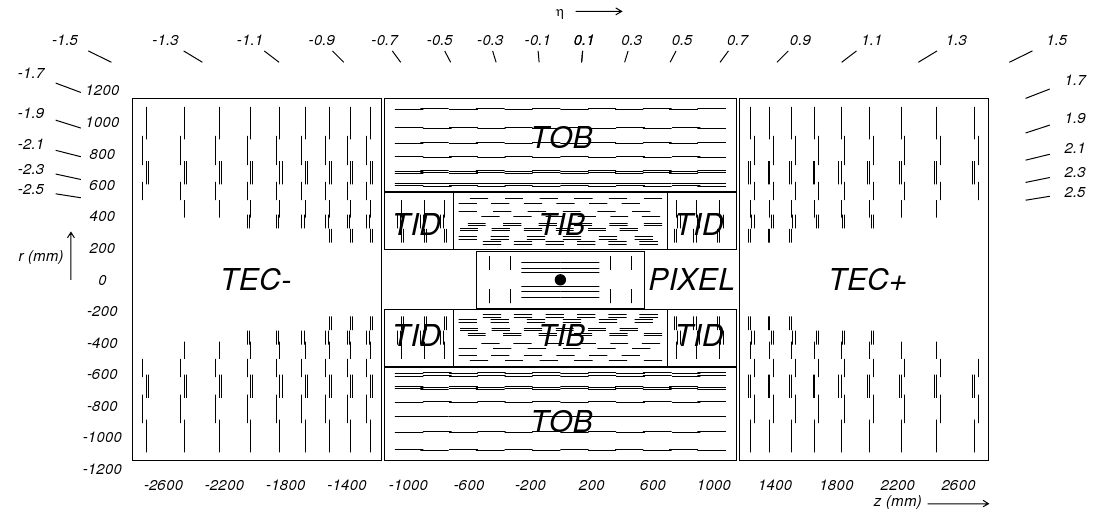
\includegraphics[width=0.8\linewidth]{figs/detector/tracker}
	\end{center}
	\caption{Schematic cross-sectional view (in the $r$-$z$ plane) of the CMS 
		tracker~\cite{cms}. The tracker modules are indicated by the black line 
		segments.}
	\label{fig:tracker}
\end{figure}

The pixel detector comprises 3 barrel layers and 2 endcap layers. Each pixel is 
$100~\micro\metre\times150~\micro\metre$ in size. The spatial 
resolution is approximately $10~\micro\metre$ in the {$r$-$\phi$} plane and 
$20~\micro\metre$ in the $z$ direction.

The barrel section of the strip detector comprises the Tracker Inner Barrel 
(TIB) consisting of 4 layers, and the Tracker Outer Barrel (TOB) consisting of 
6 layers. The strips range in size from $10~\centi\metre\times80~\micro\metre$ 
in the TIB to $25~\centi\metre\times180~\micro\metre$ in the TOB. The endcap 
region of the strip detector is made up of the Tracker End Cap (TEC) consisting 
of 9 disks, and the 3 Tracker Inner Disks (TID) that lie between the TIB and 
the TEC.
%strips resolution ranges between 13-47 microns

The tracker is able to record a hit of a charged particle with $\pt>1$~GeV with 
an efficiency of over 99\%. The transverse momentum resolution 
$\frac{\Delta\pt}{\pt}$ is approximately 2\% for particles with $\pt = 100$~GeV.

\subsection{Electromagnetic calorimeter}
%Designed to detect electrons and photons. Lead tungstate crystals.
%EB. EE. Preshower.
%Diagram of layout.
%How ECAL works (ECAL shower, bremmstrahlung and pair production - see Adam and 
%APP MSci course.)
%excite atoms, when de-excite emit scintillation light (blue), light hits 
%silicon 
%photodiodes which emits electrons (photoelectric effect) which is measured as 
%a current
%Resolution formula (a+b+c).

%% http://iopscience.iop.org/article/10.1088/1748-0221/9/02/C02008/pdf
%http://cms.web.cern.ch/news/crystal-calorimeter
%see explanation of avalanche photodiodes and vacuum phototriodes

The CMS ECAL consists of over 75,000 lead tungstate (PbWO$_4$) crystals. These 
are distributed in the ECAL Barrel (EB) and ECAL Endcap (EC), which cover the 
pseudorapidity ranges of $\etaabs<1.48$ and $1.48 < \etaabs < 3$, 
respectively. The ECAL is illustrated in Fig.~\ref{fig:ecal}. 
The energy resolution $\frac{\Delta E}{E}$ of the ECAL is approximately 0.3\% 
for high energy electrons.

% sandro: supermodules (red line i think), modules (4), submodules (5x2)
\begin{figure}
	\begin{center}
		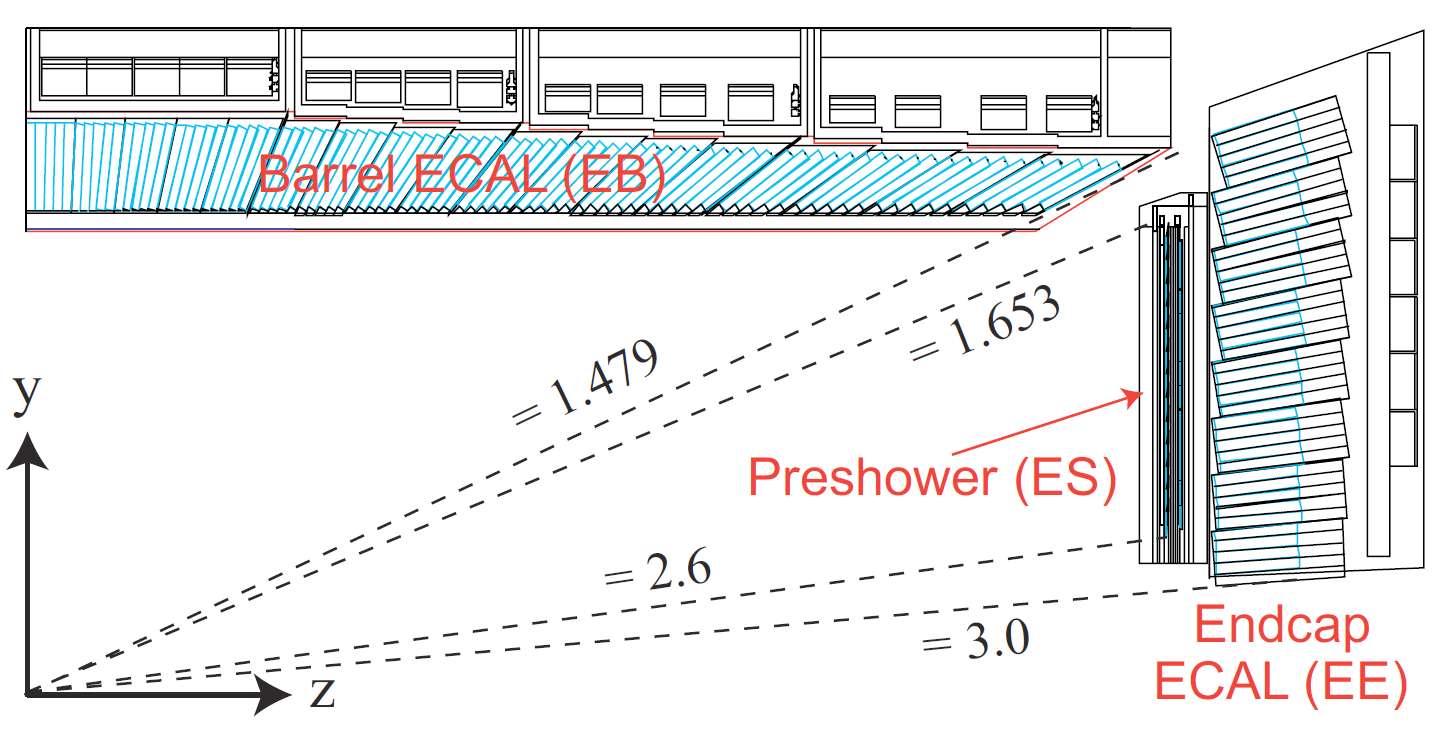
\includegraphics[width=0.7\linewidth]{figs/detector/ecal}
	\end{center}
	\caption{Schematic cross-sectional view (in the $r$-$z$ plane) of the CMS 
		electromagnetic calorimeter, showing the arrangement of crystals in the 
		barrel, 
		endcap and preshower~\cite{cms}.}
	\label{fig:ecal}
\end{figure}

The crystals in the barrel have a front-face size of 
$22~\milli\metre \times 22~\milli\metre$ and a length of 23~cm. The 
scintillation 
light produced by the electromagnetic showers is collected by silicon 
avalanche photodiodes in the barrel and vacuum phototriodes in the endcaps that 
are glued to the ends of the crystals.
% amplification/gain of 50

The ECAL Preshower (ES) detector is placed in front of the endcaps. It is 
composed of two alternating layers of lead radiator and silicon strip sensors 
and helps to distinguish between prompt photons and photons produced in the 
decays of neutral pions.%~\cite{cms}.

\subsection{Hadronic calorimeter}
%Designed to detect hadrons/jets. Brass and scintillating plastic. Photodiodes. 
%HF. Fibres.
%HB. HE. HO. HF
%Diagram of layout.
%How HCAL works (hadronic showers produce scintillation light - see Adam and 
%APP MSci course.)
%Resolution formula.

%% http://cms.web.cern.ch/news/hadron-calorimeter

The CMS HCAL is a sampling calorimeter consisting of alternating layers of 
brass absorber and plastic scintillator. The scinitillation light is collected 
by hybrid photodiodes. The HCAL is divided into the HCAL Barrel (HB), which 
covers the central region of $\etaabs < 1.4$, the HCAL Endcap (HE), covering 
the pseudorapidity range $1.3 < \etaabs < 3$, the Outer HCAL (HO), which is 
located in the barrel region behind the solenoid magnet, and the 
Forward HCAL (HF) which covers the forward region $3 < \etaabs < 5$ and is 
placed at a distance in $z$ from the interaction point of about 11~m. 

\begin{figure}
	\begin{center}
		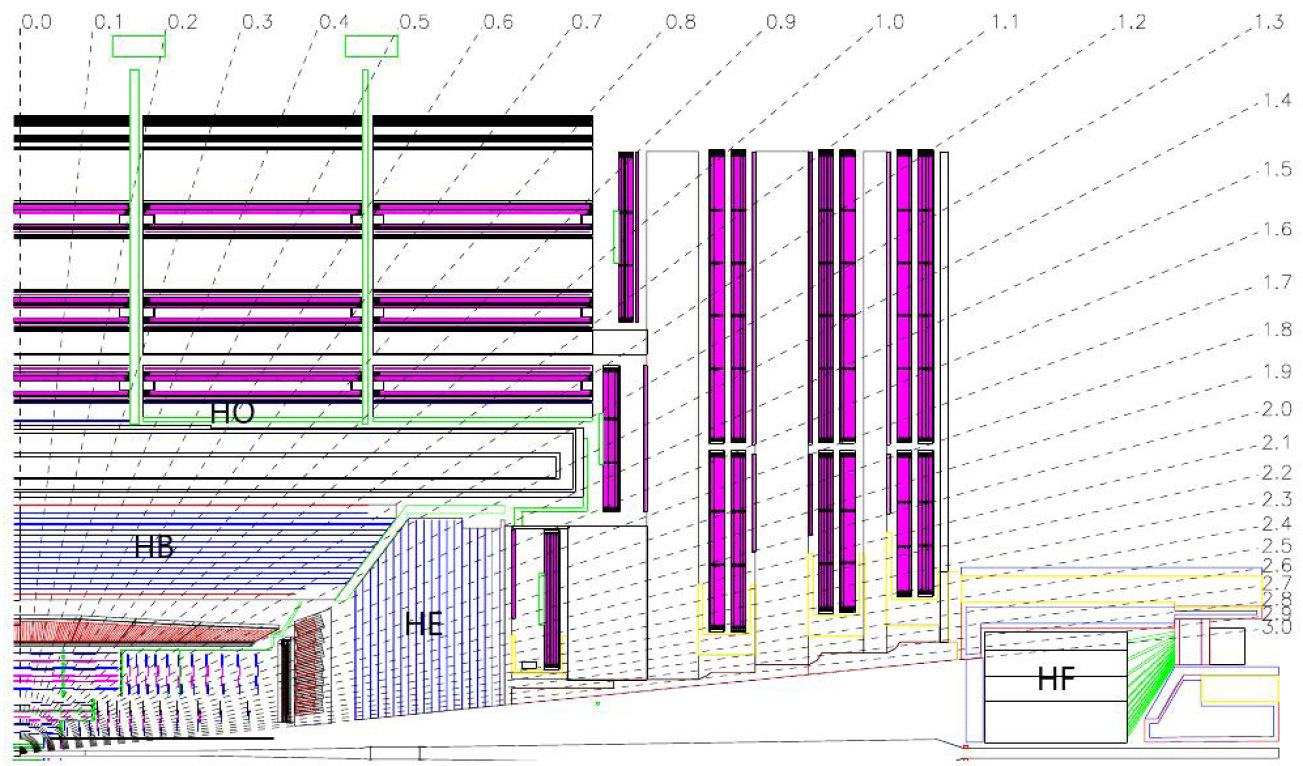
\includegraphics[width=0.7\linewidth]{figs/detector/hcal}
	\end{center}
	\caption{One quarter cross-sectional view (in the $r$-$z$ plane) of the CMS 
		detector, showing the location of the hadronic calorimeter barrel (HB), 
		endcap 
		(HE), outer (HO), and forward (HF) regions~\cite{cms}.}
	\label{fig:hcal}
\end{figure}

The calorimeter cells in the HB have dimensions of $\Delta\eta\Delta\phi = 
0.087 \times 0.087$. % sizes varies with eta (gets larger)
The purpose of the HO is to capture hadronic showers that leak past the HB, 
increasing its effective thickness to over 10 interaction lengths. 
% HO increases interaction length of HB from 5-10 to 11
The HF is designed to capture very forward particles and, due to the increased 
particle fluxes in this region, is instead made of steel absorber and quartz 
fibers. In this case hadronic showers produce Cerenkov radiation that is 
detected by photomultiplier tubes. 
% quartz more radiation resistant than plastic

The energy resolution of the ECAL and HCAL combined has been measured in a test 
beam and can be parameterised as~\cite{calo-resolution}:
\begin{equation}
\left(\frac{\Delta E}{E}\right)^2 = \left(\frac{84.7\%}{\sqrt{E}}\right)^2 + 
(7.4\%)^2 \, ,
\end{equation}
where $E$ is the energy of the incident particle in units of GeV.

\subsection{Magnet}
%Just one or two short paragraphs.
%See Marco-Andrea, Citron, Baber, Pesaresi.
The CMS magnet is a superconducting solenoid magnet producing a 3.8~T magnetic 
field. It is made of niobium-titanium and has a length of 12.9~m and a diameter 
of 6~m. A high magnetic field strength was chosen to provide a good charge 
identification and transverse momentum resolution even for very energetic 
charged particles. The return yoke of the magnet is made of steel and is 
interleaved with the muon chambers.

%The superconducting coil rests inside a vacuum chamber and is cooled to 4.5K 
%using liquid helium

%Citron: The design specifications of the solenoid magnet are driven by the 
%desire to unambiguously determine the sign of muons with momentum ∼ 1 TeV. 
%This %requires a resolution of 10\% at p = 1TeV.

%purpose (bend tracks, expecially high momentum)
%size, 3.8 T, superconducting magnet, niobium-titanium
%return yoke (purpose see below plus stop punch through hadrons)

%The operating field was scaled down to 3.8 T instead of the full design 
%strength in order to maximize longevity
%The operating current for 3.8 T is 18,160 A, giving a stored energy of 2.3 GJ.
% superconducting = can carry larger currents and therefore large mag field

%return yoke: 12-sided iron structure that surrounds the magnet coils and 
%contains and %guides the field
% Pes: return and containment of the magnetic field
% return flux is 1.8 T

\subsection{Muon system}
%Adam: As muons are heavier than electrons, they are minimally ionising and 
%lose little energy through bremsstrahlung. They therefore mostly pass through 
%the ECAL and HCAL. As muons are a key component of many electroweak decays, 
%CMS %has a dedicated muon system interleaved with the iron return yoke 
%%surrounding %the solenoid.
%DT (MB), CSC (ME), RPC.
%Diagram of layout.
%Momentum resolution with tracker 1\%.
% keep it short/concise (Citron, MA)
The CMS muon system employs three types of gaseous ionisation detectors, that 
are placed in layers interleaved with the magnet return yoke. It consists of 
the Muon Barrel (MB), covering the pseudorapidity range $\etaabs < 
1.2$, and the Muon Endcap (ME), covering the range $0.9 < \etaabs < 2.4$. The 
layout of the muon system is illustrated in Fig.~\ref{fig:muondet}.

\begin{figure}
\begin{center}
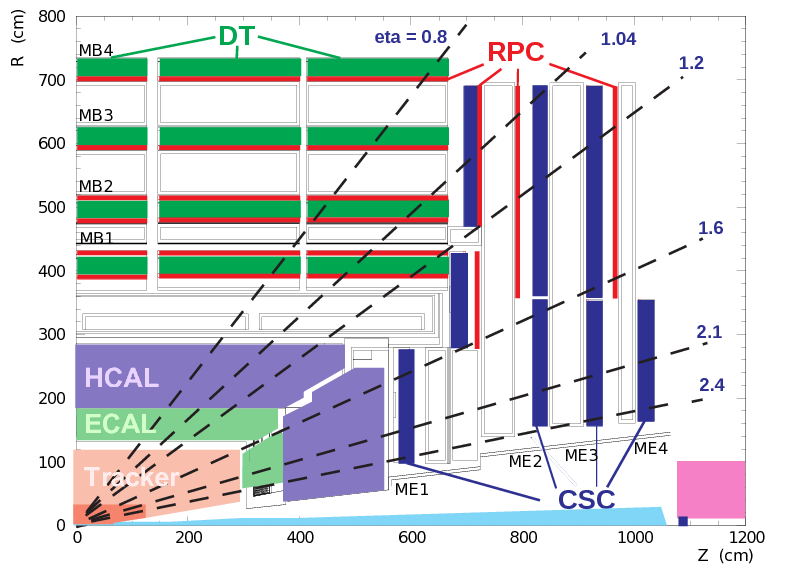
\includegraphics[width=0.7\linewidth]{figs/detector/muondet}
\end{center}
\caption{One quarter cross-sectional view (in the $r$-$z$ plane) of the CMS 
muon system, showing the location of the drift tube (DT), cathode strip chamber 
(CSC) and resistive plate chamber (RPC) subsystems~\cite{cms}.}
\label{fig:muondet}
\end{figure}

The barrel region is made up of drift tubes (DT). Cathode strip chambers (CSC) 
instrument the endcaps where particle fluxes are higher. Resistive plate 
chambers (RPC) are used in both the barrel and endcap regions for redundancy. 
These have a coarser spatial resolution than DTs and CSCs but provide a faster 
temporal resolution, which is beneficial for triggering purposes and for a 
precise bunch crossing determination.

%The muon momentum is measured in the inner tracker and in the return flux; the 
%muon momentum resolution of the combined measurement is 1\% for |eta| < 0.8 
%and pT = 10 GeV (pT/pT = 4% for pT = 1 TeV). The resolution is degraded in the 
%%endcap regions (2-10%).
The transverse momentum of muons is measured via a combination of the muon 
system and the tracker. The momentum resolution $\frac{\Delta\pt}{\pt}$ of the 
combined measurement is approximately 1\% (4\%) in the region $\etaabs<0.8$ for 
muons with a transverse momentum of 10~(1000)~GeV.

\subsection{Trigger and data acquisition}
%40 MHz. L1 trigger. HLT.
% 1 MB per event -> 40 TB per second
The crossing of proton bunches at the LHC occurs at a rate of 40~MHz. This 
results in a potentially large amount of data that is not computationally 
feasible to process and store. In any case, the majority of collisions consist 
of QCD soft scattering processes rather than electroweak or BSM processes and 
can largely be discarded. A two-level triggering system is employed in the CMS 
experiment, consisting of a hardware-based Level 1 (L1) trigger (L1T) and a 
software-based High Level (HL) Trigger (HLT), to select events of interest such 
as those containing a large amount of missing energy or particles with large 
transverse momentum, and reduce the data rate to a more manageable $\sim$1~kHz.

%reduce granularity/resolution information
% hardware (FPGAs)
The Level 1 trigger is based on custom electronic systems and reduces the event 
rate to 100~kHz. To meet the latency budget of $3.2~\micro\second$, it employs 
coarse information from the calorimeters and muon detectors and simplified 
reconstruction algorithms. The L1T consists of an L1 calorimeter trigger which 
reconstructs electrons, photons, jets and missing transverse energy, and an L1 
muon trigger which reconstructs muons. These objects are passed to the L1 
Global Trigger which makes a decision to pass the event to the HLT based on 
whether the objects satisfy certain requirements on quantities such as the 
transverse momentum.

% several thousand CPUs
% L1 to HLT via fibre optic cables
% software (C++)
Events that are accepted by the L1T are passed to the high level trigger, which 
reduces the data rate down to $\sim$1~kHz. The HLT consists of a large farm of 
processors located at ground level. It uses full-granularity data from all 
subdetectors, including the tracker, to reconstruct objects with a performance 
that is close to that offline. The HLT is discussed further in 
Sec.~\ref{sec:analysis-trigger}.

%The GRID computing infrastructure allows the offline reconstruction and 
%processing to be distributed to dedicated computing sites across the globe
Events that are accepted by the HLT are reconstructed and stored using the 
Worldwide LHC Computing Grid (WLCG), a distributed computing system making use 
of a tier hierarchy~\cite{grid}. This allows the data (and simulation samples) 
to be processed, stored and analysed at multiple sites across the world.

%\subsection{Software and computing}
% CMSSW
%Computing tiers.
% https://cms.cern/detector/computing-grid

%\subsubsection{L1 trigger upgrade and my service work?}
%Not sure yet. Look at Adam, Matt, Jad.

\section{Event reconstruction}
\label{sec:detector-reconstruction}
\begin{comment}
Intro: need to put together the things observed in the detector to reconstruct 
the objects.

Object reconstruction/identification (requires revision).
Tag and probe.
vertexing/tracking, btagging, PF, antikt.
PU subtraction, isolation, cross-cleaning.
MC corrections (JECs, PU, btagging, lepton ID, etc.).

Mention objects/working points used in analysis as you go along. Maybe summary 
table like Matt. Actually maybe include this in analysis chapter (see Adam).
\end{comment}
%need to put together the things observed in the detector to reconstruct the 
%objects.
The hits and energy deposits in the CMS subdetectors need to be combined in 
order to reconstruct and identify all physics objects in an event such as 
electrons, muons, photons, hadrons, jets and missing energy. The event content 
can then be analysed further for the purpose of, for example, a search for BSM 
physics, as will be discussed in Chap.~\ref{chap:analysis}. The various 
reconstruction and identification algorithms are described in this section.

\subsection{Particle flow algorithm}
%Need to decide where to put this. Not clear on the connection between object 
%reconstruction and particle flow.
%Resources: Particle Flow paper, Particle Flow summary.
Electrons, photons, muons, charged hadrons and neutral hadrons are all 
reconstructed by the Particle Flow (PF) algorithm by combining information from 
all subdetectors~\cite{particleflow17}. 

First, tracks in the inner tracker and 
in the muon system are reconstructed, and energy deposits in the calorimeter 
cells are grouped into clusters. Muons are identified by matching tracks in the 
inner tracker and in the muon system. 
%These are removed for subsequent steps.
Electrons are then identified by matching inner tracks with compatible energy 
clusters in the ECAL. Charged hadrons are similarly identified through the 
matching of tracks with HCAL clusters.
%AE: Electrons and hadrons are typically differentiated based on the proportion
%of energy they deposit in the ECAL or HCAL
Finally, photons are identified by energy deposits in the ECAL that are not 
matched to any tracks, and neutral hadrons are similarly identified by 
unmatched HCAL clusters.

More details on the reconstruction of each of these objects are provided in the 
following sections. These \textit{PF particles} then form the basis for the 
reconstruction of jets and missing energy.

%maybe make tracks, electronsandphotons, muons subsubsections.

\subsection{Tracks and vertices}

% todo maybe shorten this section given all other object reco sections are 
%quite short

%Combinatorial track finder (CTF), Kalman filter.
%Primary vertex. PU vertices. Secondary/displaced vertices (b quarks) found in 
%subsequent levels of reconstruction.
%Efficiencies.
%Isolated tracks? (when talking about analysis objects).
The trajectories of charged particles in the tracker are reconstructed using 
the Combinatorial Track Finder (CTF) algorithm~\cite{track-vertex}. 
A similar procedure is followed to reconstruct tracks in the muon system.
The algorithm starts by forming initial track candidates, or \textit{seeds}, 
based on 
combinations of two or three hits in the inner layers of the tracker. A seed 
defines an initial estimate of a particle's helical trajectory and is required 
to be compatible with originating from the collision region. Using a Kalman 
filter, compatible hits from successive tracker layers are added to the track 
and the trajectory parameters are updated at each layer. Another Kalman filter 
is then used to fit the final sequence of hits and smooth the estimated 
trajectory. 
%to account for a potential in the beam spot constraint imposed on the seeds
Finally, various quality criteria are imposed on the reconstructed 
tracks, such as a minimum on the number of layers that have hits and the 
$\chi^2$ value of the fit, to discard fake and duplicate tracks. The whole 
process is repeated six times, with the hits associated with reconstructed 
tracks removed in subsequent iterations. The track finding efficiency of the 
CFT algorithm is approximately 95\% for pions with $\pt>100$~GeV travelling 
through the barrel region, and almost 100\% for muons.
%As muons do not undergo nuclear interactions with the tracking detector, they 
%are reconstructed with near full efficiency across the entire tracking 
%detector.

% two tracks are duplicate if share >19 percent of hits

% Kalman filter accounts for uncertainties such as due to energy loss (brems) 
%or multiple scattering

%This algorithm follows an iterative tracking process in which a collection of 
%tracks is built up over six iterations of the reconstruction procedure.
% first iteration will find easy tracks such as high pt and close to 
%interaction point, further iterations find harder tracks such as low pt and 
%far from beam spot

The reconstructed tracks are then clustered to identify the locations of the 
various proton-proton interactions, known as interaction 
vertices~\cite{track-vertex}. This is done using a deterministic annealing 
algorithm. For a given cluster of tracks, the position of the associated vertex 
is then estimated by means of an adaptive vertex fitter.
% DA: see description on page 46 of vertex and tracking paper
The location of the \textit{hard scatter}, referred to as the \textit{primary 
vertex}, is defined by the vertex with the largest sum of the squared 
transverse momenta of the associated tracks. The other vertices are attributed 
to pileup. Secondary vertices from the decays of long-lived particles such as 
b-hadrons may be identified in further reconstruction steps.
%hard scatter: “Hard” means large momentum transfereither a violent scatter or 
%creation of a system of large mass

%The efficiency increases to close to 99.9% for events with ≥ 3 tracks. The 
%%vertex resolution reaches ∼10 μm in x, y and ∼15 μm in z with > 40 
%%reconstructed tracks.

\subsection{Muons}
%Global and tracker muons.
%%% AN-2008/097 
%%% https://twiki.cern.ch/twiki/bin/view/CMSPublic/WorkBookMuonAnalysis
Two different approaches are followed to reconstruct muons. The first is an 
outside-in algorithm that begins with a track in the muon system and attempts 
to match it with a compatible track in the inner tracker. If a match is found, 
a fit to the hits in both detectors is performed using a Kalman filter to 
determine the muon's trajectory. Muons that are reconstructed in this way are 
called \textit{global muons}. The second approach is an inside-out algorithm 
that begins with a track in the tracker and extrapolates it and attempts to 
find at least one compatible hit in the muon system. These tracks are referred 
to as \textit{tracker muons}.
%The second approach considers all tracker tracks to be potential muons and
%extrapolates those tracks to the calorimeters and the muon system; if at least
%one muon segment corresponds to the extrapol

The tracker muon algorithm is particularly useful for reconstructing muons with 
low transverse momentum ($\pt \lesssim 5$~GeV) as these often do not leave 
enough hits in the muon system to be reconstructed as muon tracks. The global 
muon algorithm, on the other hand, provides an improved momentum resolution 
for high \pt muons as hits over a larger range are employed and the full 
bending power of the CMS magnetic field is taken advantage of.

\subsection{Electrons and photons}
%\subsubsection{Tag and probe/corrections}
%build clusters (narrow in eta, wide in phi because of brem/conversion)
%gsf tracking for electrons because of brem
%match clusters with tracks, no track for pho
Interactions with the tracker material cause electrons to lose energy via 
bremsstrahlung radiation and photons to convert into electron-positron pairs. 
This leads to electromagnetic showers in the ECAL that tend to be spread out 
(in the case of electrons, the energy deposits are narrow in $\eta$ and wide in 
$\phi$). The energy deposits in the ECAL crystals that are within a certain 
window in $\eta$ and $\phi$ of a local maximum seed crystal are aggregated to 
form \textit{superclusters}. 
% see diagram in Citron
Instead of using a Kalman filter, the electron trajectories in the tracker are 
reconstructed using a Gaussian Sum Filter (GSF) algorithm, which is able to 
account for large energy losses due to bremsstrahlung radiation~\cite{gsf}. 
Electrons are then identified by an ECAL supercluster that is compatible with a 
GSF track, whereas photons are identified via unmatched superclusters.

%http://www-library.desy.de/preparch/desy/proc/proc10-04/P16.pdf

%https://en.wikipedia.org/wiki/Bremsstrahlung
%https://en.wikipedia.org/wiki/Synchrotron_radiation
%https://en.wikipedia.org/wiki/Pair_production

%% electrons lose on average 33% of energy before reaching ECAL
%% around 50% of photon convert before reaching ECAL

%in barrel: find local 5x1 maximum, then cluster with other 5x1 dominoes 
%looking in a phi window of pm17 crystals.

%These reconstructed superclusters are used in the reconstruction of all
%electrons and photons in the event

%photons is measured best using the energy contained in a 5 × 5 crystal matrix 
%around the seed crystal, corrected for the lateral leakage correction f(η) and 
%for module border effects

%bremsstrahlung, which has a non-Gaussian loss distribution.
%As the Kalman filter that is used in track reconstruction assumes Gaussian 
%%%energy losses, another specialist track reconstruction for electrons is 
%%employed

%Hits in both the first and second layers compatible with a supercluster are 
%%%then used as seeds for dedicated electron track reconstruction, performed 
%%%%using a Gaussian sum filter (GSF) algorithm [80], which performs better 
%%%%than a 
%%%%%Kalman Filter for tracks with significant energy loss.

\subsection{Jets}
\label{sec:detector-jets}
%Briefly describe what a jet is (hadronisation, tight cone of particles [MA]).
%antikt algorithm. Infrared and collinear safe.
%Inputs are PF candidates. Pileup subtraction (not just here but for all 
%objects).

% if you need refresher in understanding algorithm, see sandro p100

%references: towards jetography
% antikt: http://iopscience.iop.org/article/10.1088/1126-6708/2008/04/063/pdf

% see example of infrared and collinear unsafety
% https://arxiv.org/pdf/hep-ex/0005012.pdf

% in the central region, typically have a fractional composition of: 65% 
%%charged hadrons, 25% photons and 10% neutral hadrons.

% emission of soft gluon occurs 
% fragments = showers (emits soft qcd radiation)
Due to the nature of the strong force, when a quark or gluon is produced it 
immediately fragments and hadronises, leading to a collimated spray of hadrons 
known as a \textit{jet}. In this search, jets are reconstructed by clustering 
Particle Flow particles using the \antikt sequential recombination 
algorithm~\cite{antikt}. This algorithm is both infrared safe and collinear 
safe, 
meaning that the set of reconstructed jets remains unchanged in the case of a 
soft gluon emission or a splitting of a gluon into two collinear gluons. 
%jets can undergo soft gluon radiation of arbitrarily low energy gluons with a 
%high probability.

A sequential recombination algorithm is based on a distance between pairs of 
particles $d_{ij}$ and between particles and the beamline $d_{iB}$. These are 
defined for the \antikt algorithm as:
\begin{equation}
d_{ij} = \mathrm{min} \left( \frac{1}{\pt_i^2}, \frac{1}{\pt_j^2} \right) 
\frac{\Delta R_{ij}^2}{R^2}
\end{equation}
\begin{equation}
d_{iB} = \frac{1}{\pt_i^2}
\end{equation}
where $\pt_i$ is the transverse momentum of particle $i$, 
$\Delta R_{ij}=\sqrt{(\eta_i - \eta_j)^2 + (\phi_i - \phi_j)^2}$ is the 
distance between particles $i$ and $j$ in the {$\eta$-$\phi$} plane, and 
$R=0.4$ defines the radius of the jet in {$\eta$-$\phi$} space.

The algorithm begins by computing all distances $d_{ij}$ and $d_{iB}$. If one 
of the $d_{ij}$ is the smallest distance of all, particles $i$ and $j$ are 
combined into a new particle (or pseudo-jet) by taking the vector sum of their 
momenta. 
If instead one of the $d_{iB}$ is the smallest distance, particle $i$ is 
classified as a jet and removed from subsequent steps. The process is then 
repeated (starting again by recomputing all distances) until no particles 
remain.

%Adam: R = 0.4 is often chosen as it contains the hadronic showers of most 
%%%quarks and gluons produced in 13 − 14 TeV proton collisions, while remaining 
%%%%insensitive to contamination from PU.
% "combining" particles means summing their three-momenta

%For the kT algorithm the exponent is chosen as p = 1, which results in jets 
%being clustered initially from the softest pseudojets to successively harder 
%pseudojets. The anti−kT clustering algorithm utilises a negative exponent p = 
%−1 which has the converse behaviour, clustering first the hardest pseudojets 
%to %progressively softer pseudojets. A special case with p = 0 is used in the 
%Cambridge/Aachen algorithm, in which case only the distance information 
%between %the pseudojets is utilised which is of interest in the clustering of 
%%boosted %jets. Jet clustering within CMS is primarily performed by the 
%%%anti−kT 
%algorithm %due to its greater resilience to pileup and tendency to cluster 
%%circular jets.

As the jet reconstruction algorithm clusters all PF particles, isolated leptons 
and photons may be classified as jets. To avoid this, a \textit{cross-cleaning} 
procedure is performed in which reconstructed jets that are within $\Delta R < 
0.4$ of an isolated muon, electron or photon (isolation will be defined in 
Sec.~\ref{sec:detector-isolation}) are excluded from the event.

\subsubsection{Jet energy corrections}
\label{sec:detector-jecs}
%JECs. JER? applied to both data and mc
% https://arxiv.org/pdf/1607.03663.pdf
% https://arxiv.org/pdf/1107.4277.pdf
%https://twiki.cern.ch/twiki/bin/viewauth/CMS/JetEnergyScale#Documents_and_Analysis
%https://twiki.cern.ch/twiki/bin/view/CMS/IntroToJEC
% see also Dunne 1st year report
The energies of reconstructed jets typically differ from the true energy of the 
original quark or gluon due to a non-uniform and imperfect resolution of the 
detector. The measured transverse momentum of a jet 
$p_{\mathrm{T}}^{\mathrm{raw}}$ is corrected to account for this via a sequence 
of multiplicative correction factors (the output of each step is the input to 
the next) according to~\cite{jec}:
\begin{equation}
p_{\mathrm{T}}^{\mathrm{corr}} =  p_{\mathrm{T}}^{\mathrm{raw}} 
C_{\mathrm{offset}} C_{\mathrm{sim}} C_{\mathrm{rel}} C_{\mathrm{abs}} 
\end{equation}
%\begin{equation}
%p_{\mathrm{T}}^{\mathrm{corr}} =  p_{\mathrm{T}}^{\mathrm{raw}} 
%C_{\mathrm{offset}}(p_{\mathrm{T}}^{\mathrm{raw}}) C_{\mathrm{sim}} 
%(p_{\mathrm{T}}', \eta) C_{\mathrm{rel}} (\eta) C_{\mathrm{abs}} 
%(p_{\mathrm{T}}'')
%\end{equation}
The first correction is an offset correction $C_{\mathrm{offset}}$ that 
subtracts the energy contributions from electronics noise and particles 
originating from pileup vertices. 
% CHS, rho-area
% CHS + offset = double counting?
The second is a correction derived from simulation $C_{\mathrm{sim}}$ and is 
given by the ratio of reconstructed and generator-level jet \pt. It is derived 
as a function of \pt and $\eta$. 
% MC correction removes the bulk of the non-uniformity in η and the 
%non-linearity in pT
The third and fourth components are the relative and absolute corrections, 
$C_{\mathrm{rel}}$ and $C_{\mathrm{abs}}$, that are used to correct for 
remaining small discrepancies in the jet energies measured in data as a 
function of $\eta$ and \pt, respectively. 
% are applied only in data and 
The overall correction factor (given by the product of the four correction 
terms) is found to be in the range of 1-1.1 (depending on $\eta$) for jets with 
transverse momentum $\pt=100$~GeV.
% vs eta: kinda flat with spikes at eta=2 (transition region)

\subsubsection{b-tagging}
\label{sec:detector-btagging}
%Identification of jets originating from bottom quarks.
%see btagging CMSDAS Introduction.pdf
%eg slide 11 how eff varies with pt and eta, ROC curves, etc.
%put a plot.

% btagging paper 17...pdf (latest BTV 36fb paper)
%https://twiki.cern.ch/twiki/bin/view/CMSPublic/WorkBookBTagging
%https://twiki.cern.ch/twiki/bin/viewauth/CMS/SWGuideCMSDataAnalysisSchoolBTaggingExercise

% sec 4.3 describes briefly secondary vertex reconstruction algos (IVF)
%https://arxiv.org/pdf/1712.07158.pdf

%specifically a feed-forward multilayer perceptron with one hidden layer

%Adam: In a wide range of SUSY models the decay via top quarks is favoured over 
%%%other, lighter quarks
% also DM+tt/bb
% also ttbar background
A number of BSM models include the associated production of, or decays to, top 
and bottom quarks. It is therefore advantageous to able to identify jets that 
originate from a bottom quark, a process known as \textit{b-tagging}.

%long lifetime: τ≈1.5 ps, cτ≈450 μm, γβcτ≈1.8 mm @ 20 GeV
%large mass: ~5 GeV
%high track multiplicity: ~4–5
%tau=1.5ps travel betagammactau 1.8mm
% c lifetiem: 1 ps
Hadrons containing bottom quarks have a lifetime of about 1.5~ps, and therefore 
travel a few millimetres before decaying. This can be observed experimentally 
as a jet containing several tracks that originate from a \textit{secondary 
vertex} that is displaced from the primary vertex.

% impact parameter, which is defined as the distance between the primary vertex 
%and the tracks at their points of closest approach
% example variables: SV 2D flight distance, SV mas, number of SVs, 3D IP of 
%first four tracks, track pt, distances between tracks and jet axis
% CSV doesn't need there to be a SV (have other variables)
The Combined Secondary Vertex (CSV) algorithm is employed to perform 
b-tagging~\cite{btagging}. It consists of an artificial neural network taking a 
number of input variables related to the secondary vertex (such as the 
displacement and invariant mass) and the displaced tracks (such as the impact 
parameters). The output discriminator of the neural network is a value between 
0 and 1 which can be thought of as the probability that the given jet 
originates from a bottom quark. Figure~\ref{fig:btagcsv} demonstrates the 
ability of the algorithm to discriminate between jets originating from b quarks 
and jets originating from gluons or u, d, s or c quarks. A threshold for the 
discriminator value may be chosen according to the desired b-tagging efficiency 
and fake rate.
% at least two tracks per jet required
% if two tracks compatible with K-short meson reject (lifetime ~10 ps)

\begin{figure}
\begin{center}
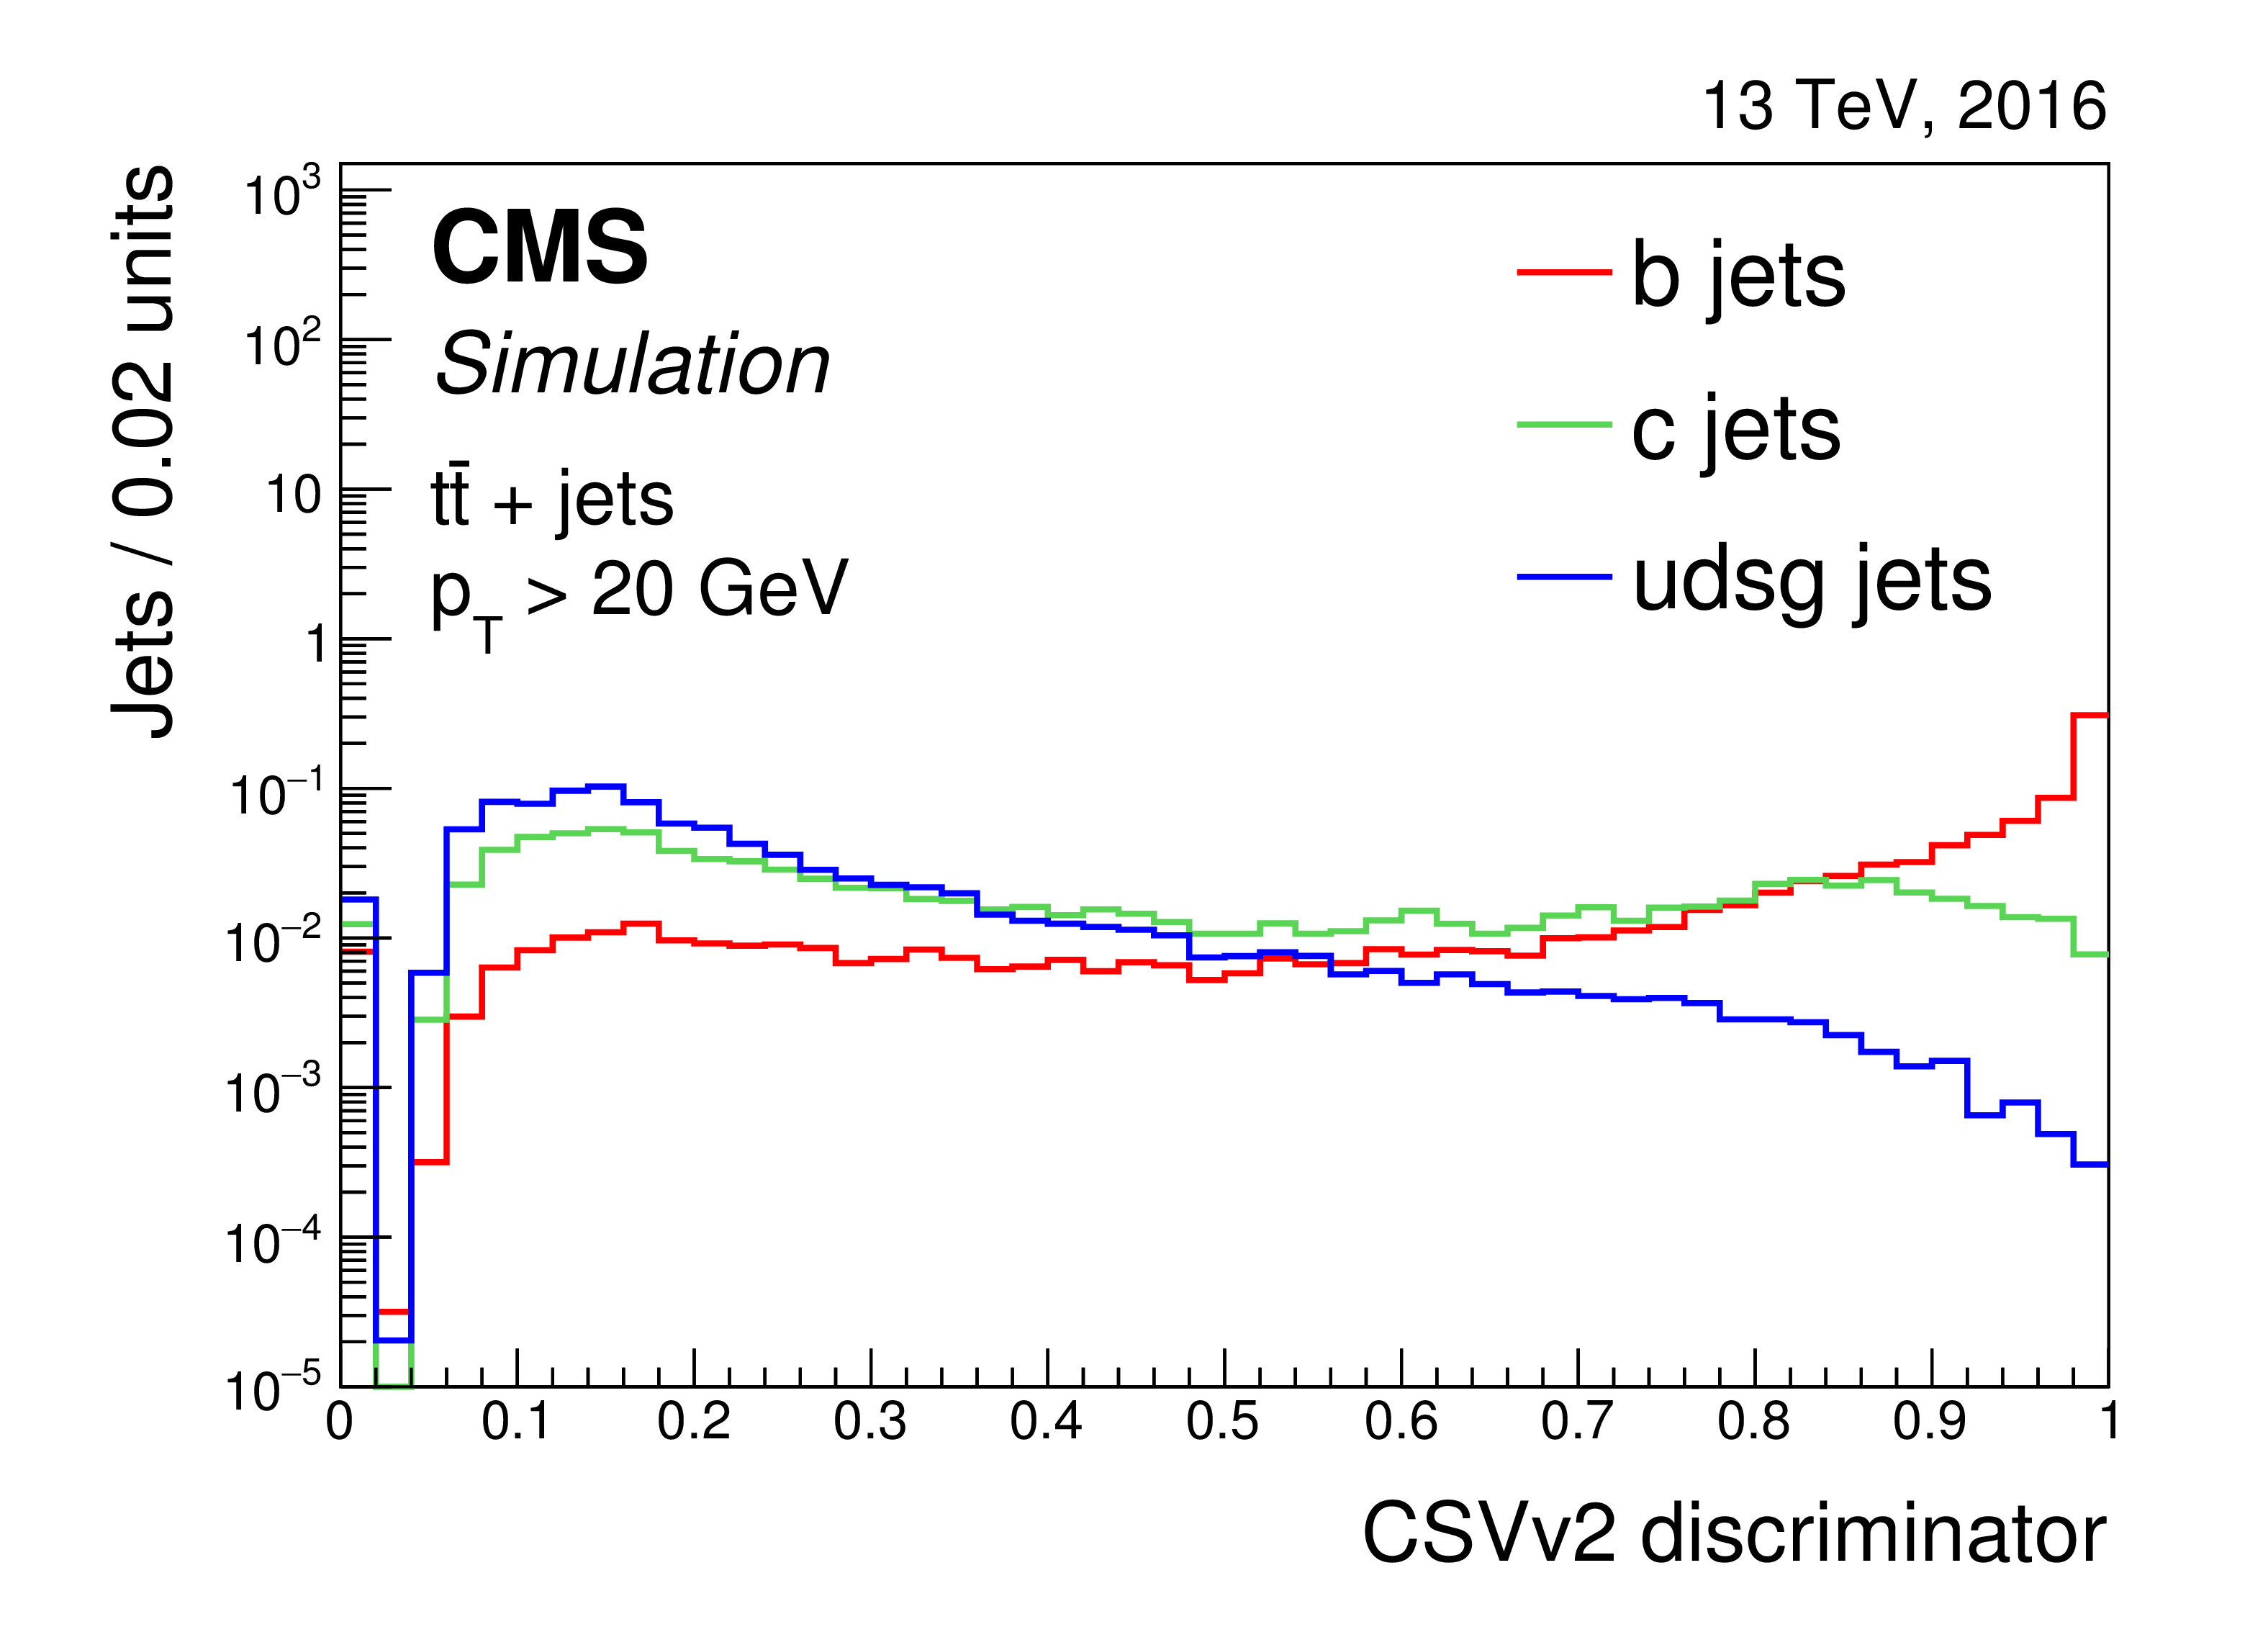
\includegraphics[width=0.8\linewidth]{figs/detector/btagcsv}
\end{center}
\caption{Distribution of the discriminator value of the CSV b-tagging algorithm 
for jets of different flavours in simulated \ttbar events~\cite{btagging}. Jets 
without at least two tracks are assigned a default value of -1 and are included 
in the first bin, which contains the underflow entries.}
\label{fig:btagcsv}
\end{figure}

\subsection{Isolation}%, pileup subtraction and jet cross-cleaning}
\label{sec:detector-isolation}
%Define relative and mini-isolation.
%Define pileup subtraction - effective rho area, delta beta?
% CAREFUL: OVERLAP WITH phys obj SECTION IN ANALYSIS CHAPTER?
It is often important to identify \textit{prompt} leptons and photons, which 
are produced in the hard process, %at the primary interaction vertex, 
as opposed to non-prompt 
particles that are the products of in-flight decays within jets. 
% basically whether from hard scatter process or decay of random hadron in jet
This is 
accomplished by measuring the \textit{isolation}, which is a measure of the 
activity around a particle. The isolation of a particle is defined as the ratio 
of the total transverse momentum of other particles within a certain distance 
$\Delta R$, and the transverse momentum of the particle itself. A particle is 
considered to be isolated if its isolation value is below a defined threshold.

In this search, two types of isolation are utilised, which differ in the size 
of the isolation cone $\Delta R$. One is referred to as \textit{relative 
isolation} \reliso, in which a fixed cone size of $\Delta R = 0.3$ is used. The 
other is \textit{mini-isolation} \miniiso, in which the cone size depends on 
the momentum of the particle, varying from $\Delta R = 0.2$ for $\pt < 50$~GeV 
to $\Delta R = 0.05$ for $\pt > 200$~GeV. This improves the efficiency of 
identifying energetic leptons from the decays of highly boosted particles such 
as top quarks. 
% and W bosons? if W and "+jets" are close
% but higher fake rate (remember we saw more qcd)

The total energy contained within the isolation cone (the numerator of the 
isolation variable) must be corrected to account for pileup, which would 
otherwise falsely increase the isolation value and lead to a loss in 
identification efficiency. This is done by ignoring charged particles that 
don't originate from the primary vertex, and subtracting the neutral pileup 
contribution, which is estimated as $\rho \Delta R$, where $\rho$ is the 
average transverse energy density of all neutral particles in the event 
measured across the entire detector.
%"density is "per unit area", "area" being in eta-phi space
%charged hadrons identified as originating from the primary vertex, neutral 
%hadrons, and photons.
% SANDRO p93
% The rho value has units of ET /area: in order to derive an isolation 
%correction, it must be multiplied times the geometrical area of the isolation 
%cone but this computation is complicated by the detector geometry. An eective 
%area Ae f f is defined as the slope of a linear fit of the average isolation 
%of photon objects versus rho, excluding veto regions. A detailed description 
%of that method will be provided in Section 3.3.3

% page 27 https://arxiv.org/pdf/1502.02702.pdf
%rho*Aeff, where rho is the median of the transverse energy density per unit 
%area in the event [26] and Aeff is the area of the isolation region weighted 
%by a factor that takes into account the dependence of the pileup transverse 
%energy density on pseudorapidity. The effective areas have been determined in 
%gamma + jet events.

% eff area = see sandro p85
% Baber calls it "footprint"

%baber p84-85
%run1: median(pt/A) of all kt jets (which cluster all soft stuff) 
%https://arxiv.org/pdf/0707.1378.pdf
%run2: median energy density of PF candidates within grid of cells with length 
%0.55
%rho subtraction: shouldn't subtract charged pileup particles? - i guess just 
%sum up energies of neutral particles - yes (see Baber and Citron)

\subsection{Energy sums}
\label{sec:detector-energysums}
%CAREFUL: OVERLAP WITH ENERGY SUMS SECTION IN ANALYSIS CHAPTER?
%Define HT, MHT and MET. At some point (maybe near the beginning) explain why 
%we use  the transverse plane (initial momentum is zero, whereas it isn't in 
%the longitudinal plane).
%Neutrinos do not interact in particle detectors, and therefore escape 
%undetected. Their presence can be inferred by the momentum imbalance of the 
%visible particles in an event.
The production of massive supersymmetric 
particles results in a large transfer of energy to final state particles. 
In addition, weakly interacting particles such as the LSP cannot be detected 
directly, but their presence can be inferred by the transverse momentum 
imbalance of the observed particles. The total energy and missing energy in an 
event are therefore useful variables in characterising BSM processes. 

A measure of the transverse momentum of the invisible system in an event is 
provided by the negative vector sum of the transverse momenta of all Particle 
Flow particles in the event, known as the \textit{missing transverse momentum} 
or \textit{missing transverse energy}:
\begin{equation}
\bm{\cancel{E}}_\mathrm{T} = - \sum_{\mathrm{particles}} \bm{p}_\mathrm{T} \, .
\end{equation}
%Type-1 corrections.
% see MA for type-0 (pileup)
%METcorr = MET + Sum(jet pt) - Sum(jet pt corr)
%basically remove original jet pt (which is equal to sum of constituents pt) 
%%%and include corrected jet pt
% or in other words, you can scale all constituents pt by same jet energy 
%correction
%The jet energy corrections described in Sec.X are propagated as a correction 
%to the \met value 
This is calculated after the application of the jet energy corrections 
described in Sec.~\ref{sec:detector-jecs}.

%Adam: energy sums that take only jets as input,
%which are typically better understood and calibrated than each unclustered PF 
%%%candidate.
%To gain a measure of the scale of hadronic energy in an event, the HT variable
A similar quantity that is based only on the jets in the event can be defined 
as:
\begin{equation}
\bm{\cancel{H}}_\mathrm{T} = - \sum_{\mathrm{jets}} \bm{p}_\mathrm{T} \, .
\end{equation}
The scale of hadronic energy in an event is measured by the scalar sum of the 
jets' transverse momenta:
\begin{equation}
\scalht = \sum_{\mathrm{jets}} |\bm{p}_\mathrm{T}| \, .
\end{equation}

\section{Simulation}
\label{sec:detector-simulation}
%see 9M report
%methods of Monte Carlo event generation, hadronisation and detector simulation 
% very useful wiki (see highlights): 
%http://www.scholarpedia.org/article/Parton_shower_Monte_Carlo_event_generators
% also Sandro very detailed
% https://arxiv.org/pdf/1101.2599.pdf (generic MC simulation process)
% maltoni1 MC.pdf
% sandro p42 for minimum bias vs underlying event

%motivation
The simulation of background and signal processes is an important aspect of a 
search for new physics. The Monte Carlo (MC) method forms the basis of the 
simulation process.

%hard scatter, ME, PDF, NLO
%The Matrix Element (ME) method is based on the exact calculation of the matrix 
%elements and corresponds to the order-by-order calculation of Feynman diagrams 
%in perturbative QCD
%The state-of-the-art in the field of matrix element calculation is NLO, with 
%all the virtual loop corrections included. Loop calculations are complex and 
%they are available for a limited number of processes. For this reason 
%tree-level matrix element calculations still play an important role in the 
%simulation of events produced at hadron colliders
The first step is the generation of the hard scattering, in which constituents 
of the colliding protons interact and produce the outgoing particles. This is 
accomplished with MC event generators such as 
\textsc{MadGraph}~\cite{madgraph} and \textsc{powheg}~\cite{powheg}. 
The momenta of the colliding partons are sampled from a parton distribution 
function (PDF). 
%These distributions have been measured at lower energies and in other 
%processes and are evolved to higher scales using the QCD evolution equations 
%for parton densities
The generator also calculates, based on the Feynman diagrams of the desired 
process up to a certain order in perturbative QCD, the corresponding matrix 
elements and differential cross section. The final state particles are then 
generated according to the incoming parton momenta and the differential cross 
section.

%fragmentation/showering and hadronisation
%The hard subprocess, by definition, involves large momentum transfers and 
%therefore the partons involved in it are violently accelerated. Just as 
%accelerated electric charges emit QED radiation (photons), the accelerated 
%coloured partons will emit QCD radiation in the form of gluons. Unlike the 
%uncharged photons, the gluons themselves carry colour charges and can 
%therefore emit further radiation, leading to parton showers.
%The parton cascade is evolved down to a certain virtuality, of the order of 1 
%GeV2. After that, non perturbative effects take place and the hadronization is 
%applied.
%An initial-state shower is one that develops on an incoming parton of the hard 
%subprocess, of which there are two at a hadron collider. 
% quarks and gluons can radiate gluons, gluons can also produce qqbar pair
% hadronization process cannot be described in perturbative QCD.
%Baber: In fragmentation, a simulation of the splitting of the partons from the 
%hard scatter is performed, with the emission of soft quarks and gluons 
%continuing until the cut-off scale of QCD, ΛQCD∼ 200MeV, where calculations 
%become non-perturbative.
%(see pdf) Fragmentation functions describe how the color-carrying quarks and 
%gluons transform into color-neutral particles such as hadrons or photons.
The next step is the simulation of parton showers, that is additional QCD 
radiation emitted by the involved quarks and gluons, and the subsequent 
hadronisation in which colourless hadrons are formed according to the Lund 
string model. Any unstable particles in the event are then decayed. The 
showering, hadronisation and decay processes are performed with 
\textsc{pythia8}~\cite{pythia}.

%In addition to the hard scattering, a simulation of the underlying event, 
%multi-partonic interactions of the proton remnants, is also performed. 
%(additional parton collisions within the same protons)

%pileup, ootpu
Additional soft interactions are overlayed in each generated event to account 
for pileup. The effects from up to 12 preceding and subsequent bunch crossings 
(out-of-time pileup) are also included.

%material interaction
%The passage of the resulting particles through the CMS detector and their 
%interactions with the detector material (through ionisation and scattering) is 
%simulated with the GEANT4 tool-kit
%Finally, the response of each sub-detector, the electronics and the trigger 
%are emulated, and all energy deposits in the event are reconstructed as 
%physics objects.
Finally, the interactions of the resulting particles with the CMS detector 
(such as through ionisation and scattering) are simulated with 
\textsc{geant4}~\cite{geant}. The response of each subdetector, the electronics 
and the trigger are also emulated. The reconstruction methods described in 
Sec.~\ref{sec:detector-reconstruction} can then be applied as with real data.
% leads to energy loss https://en.wikipedia.org/wiki/Bethe_formula

\begin{comment}
{Data sets}

See Nick. MA has this in the analysis chapter.
We use data collected by the CMS during certain runs, plus simulated data of 
background and signal processes.

{Collected data}

35.9 fb-1. 2016. (This would be mentioned in the intro anyway).
Show lumi delivered/collected vs time.
Triggers/Primary Datasets.
SR and Muon CRs.

Maybe keep this chapter general, just have section on MC simulation, and 
mention which specific data and MC samples elsewhere.

{Monte Carlo simulation}

Description of madgraph, pythia, GEANT.

MC simulation data sets.
(Grid of masses and ctau, couplings used) - no need to specify grid, couplings 
mentioned in simplified models section.
See paper.

Describe weights and xs/lumi normalisation?
\end{comment}